\documentclass[11pt,a4paper]{article}

\usepackage[margin=2.1cm]{geometry}
\usepackage[T1]{fontenc}
\usepackage[utf8]{inputenc}
\usepackage{lmodern}
\usepackage{microtype}
\usepackage{amsmath,amssymb,mathtools}
\usepackage{booktabs,array,tabularx}
\usepackage{xcolor}
\usepackage{graphicx}
\usepackage{listings}
\usepackage{tcolorbox}
\tcbuselibrary{skins,breakable}
\usepackage{tikz}
\usetikzlibrary{arrows.meta,positioning,calc,decorations.pathreplacing,shapes.geometric}
\usepackage{fancyhdr}
\usepackage{hyperref}
\usepackage{enumitem}

\graphicspath{{../figures/}{figures/}{./}}

% ---- palette (matches the project notes) -----------------------------------
\definecolor{navy}{HTML}{1B365D}
\definecolor{slate}{HTML}{2C5282}
\definecolor{tint}{HTML}{F4F7FA}
\definecolor{amber}{HTML}{8A5A00}
\definecolor{ambertint}{HTML}{FFFBEB}
\definecolor{greenink}{HTML}{1E5631}
\definecolor{greentint}{HTML}{F1F8F4}
\definecolor{crimson}{HTML}{9B1C1C}

\hypersetup{
  colorlinks=true,
  linkcolor=slate,
  urlcolor=slate,
  pdftitle={Implementation Notes: A Front-Fixing Stefan Solver with Wet/Dry Coupling},
  pdfauthor={rosolver}
}

\pagestyle{fancy}
\fancyhf{}
\fancyhead[L]{\small\color{slate}\textsc{Implementation Notes: Stefan Front Tracking}}
\fancyhead[R]{\small\color{slate}\texttt{rosolver.phasechange}}
\fancyfoot[C]{\small\thepage}
\renewcommand{\headrulewidth}{0.4pt}

% ---- boxes ------------------------------------------------------------------
\newtcolorbox{setupbox}[1]{
  breakable, enhanced, colback=tint, colframe=navy, boxrule=0.8pt, arc=3pt,
  left=8pt, right=8pt, top=6pt, bottom=6pt, fonttitle=\bfseries\color{white}, title={#1}
}
\newtcolorbox{insightbox}[1]{
  breakable, enhanced, colback=ambertint, colframe=amber, boxrule=0.8pt, arc=3pt,
  left=8pt, right=8pt, top=6pt, bottom=6pt, fonttitle=\bfseries\color{white}, title={#1}
}
\newtcolorbox{resultbox}[1]{
  breakable, enhanced, colback=greentint, colframe=greenink, boxrule=0.8pt, arc=3pt,
  left=8pt, right=8pt, top=6pt, bottom=6pt, fonttitle=\bfseries\color{white}, title={#1}
}

\lstdefinestyle{py}{
  language=Python,
  basicstyle=\ttfamily\footnotesize,
  keywordstyle=\color{navy}\bfseries,
  commentstyle=\color{greenink}\itshape,
  stringstyle=\color{amber},
  showstringspaces=false,
  frame=single,
  rulecolor=\color{slate!40},
  backgroundcolor=\color{tint},
  breaklines=true,
  columns=fullflexible,
  xleftmargin=6pt,
  xrightmargin=6pt,
  aboveskip=8pt,
  belowskip=8pt
}

% ---- macros -----------------------------------------------------------------
\newcommand{\dd}{\mathrm{d}}
\newcommand{\pd}[2]{\frac{\partial #1}{\partial #2}}
\newcommand{\td}[2]{\frac{\dd #1}{\dd #2}}
\newcommand{\Ts}{T_s}
\newcommand{\Tw}{T_w}
\newcommand{\Tinf}{T_\infty}
\newcommand{\Tf}{T_f}
\newcommand{\Timp}{T_{\mathrm{imp}}}
\newcommand{\Lf}{L_f}
\newcommand{\keff}{k_{\mathrm{eff}}}
\newcommand{\mdot}{\dot m}
\newcommand{\ximp}{\xi_{\mathrm{imp}}}
\newcommand{\branch}[1]{\textsc{#1}}

\title{
  {\color{navy}\rule{\textwidth}{1.8pt}}\\[0.6em]
  {\LARGE\bfseries\color{navy} Implementation Notes}\\[0.25em]
  {\Large\bfseries\color{navy} A Front-Fixing Stefan Solver with Wet/Dry (Messinger) Coupling}\\[0.35em]
  {\large\color{slate} Moving-boundary ice growth, eq.~3.4 of the OTI equation sheet,
   implemented in \texttt{rosolver.phasechange}}\\[0.4em]
  {\color{navy}\rule{\textwidth}{0.8pt}}
}
\author{\texttt{rosolver} --- numerical modelling notes}
\date{\today}

\begin{document}
\maketitle

\begin{abstract}
\noindent The OTI equation sheet writes the ice-surface Stefan condition as a single
flux jump, eq.~(3.4). That equation is a boundary condition, not a closed model: it
contains the front speed, the surface temperature and an interior temperature gradient,
with no equation for the temperature field. These notes document the implementation that
turns eq.~(3.4) into a well-posed one-phase Stefan problem and solves it in
\texttt{rosolver}. The front is removed with the Landau (front-fixing) coordinate
$\xi=y/\delta(t)$, which makes $\delta(t)$ an explicit ODE state and enforces the Stefan
condition exactly, without latent-heat smearing. The resulting stiff ODE is integrated
with \texttt{BDF}/\texttt{Radau} or a fixed-step implicit scheme. A wet/dry surface
closure adds the Messinger rime/glaze switch: supply-limited growth with $\Ts<\Tf$ when
the impingement flux is below the surface heat-removal capacity, and energy-limited
growth with $\Ts=\Tf$ and runback otherwise. The implementation reproduces the exact
Neumann similarity solution for $h_c=0$ to a relative front error of
$1.6\times10^{-7}$, matches the quasi-steady reduction to $O(\mathrm{Ste})$, and passes
twenty-nine dedicated tests. Hybrid accretion/shedding events and a runback-film closure
with impingement enthalpy are integrated in the same framework
(Sections~\ref{sec:hybrid} and~\ref{sec:film}). A two-panel validation figure is
generated by \texttt{examples/stefan\_validation.py}.
\end{abstract}

\tableofcontents
\vspace{0.6em}
\hrule
\vspace{0.8em}

% ============================================================================
\section{Scope and problem statement}
% ============================================================================

The starting point is eq.~(3.4) of the OTI cheat-sheet,
\begin{equation}\label{eq:stefan}
  \rho_i \Lf \td{\delta}{t}
  = \keff(\phi)\left.\pd{T}{y}\right|_{\text{ice}}
  - h_c\left(\Tinf-\Ts\right),
\end{equation}
where $y$ is measured outward from the wall, $\delta(t)$ is the ice-layer thickness,
$\Ts$ is the surface temperature, and $h_c$ is the convective heat-transfer coefficient.
With the sign convention used here ($\Tw<\Ts$ on a cold wall, so $\pd{T}{y}>0$), the
equation is equivalently
\begin{equation}
  \rho_i \Lf \dot\delta
  = \keff\left.\pd{T}{y}\right|_{\delta} + h_c\left(\Ts-\Tinf\right),
\end{equation}
i.e.\ the latent heat released at the accreting surface is split between conduction into
the ice and convection to the air.

Equation~\eqref{eq:stefan} has three unknowns --- $\delta$, $\Ts$ and the gradient ---
and no temperature field. It becomes solvable only after adding:
\begin{enumerate}[leftmargin=1.4em,itemsep=2pt]
  \item the transient heat equation in the ice layer;
  \item a wall condition at $y=0$;
  \item an interface-temperature closure for $\Ts$.
\end{enumerate}

The implementation in \texttt{rosolver/phasechange.py} supplies all three and exposes two
surface closures:
\begin{itemize}[leftmargin=1.4em,itemsep=2pt]
  \item the \textbf{wet/energy-limited} closure, $\Ts=\Tf$;
  \item the \textbf{rime/glaze switch}, in which $\Ts$ is algebraic in the dry branch and
        pinned to $\Tf$ in the wet branch (Section~\ref{sec:wetdry}).
\end{itemize}

% ============================================================================
\section{The well-posed moving-boundary model}\label{sec:model}
% ============================================================================

\subsection{Governing equations}

Let $T(y,t)$ be the temperature in the ice, $0<y<\delta(t)$. The model is the one-phase
Stefan problem
\begin{align}
  \rho_i c_p \pd{T}{t} &= \pd{}{y}\!\left(\keff(\phi)\,\pd{T}{y}\right),
     && 0<y<\delta(t), \label{eq:heat}\\
  T(0,t) &= \Tw, && \text{(cold wall)} \label{eq:wall}\\
  T(\delta,t) &= \Ts(t), && \text{(surface continuity)} \label{eq:surfT}\\
  \rho_i \Lf \dot\delta
     &= \keff\left.\pd{T}{y}\right|_{\delta}
        + h_c\left(\Ts-\Tinf\right). && \text{(Stefan jump)} \label{eq:stefanjump}
\end{align}
The wall may also be a Robin condition; a Dirichlet wall is used here because it is the
setup of the SnowTek/WINICE benchmarks.

For a cold wall and a cold ambient, $\Tw<\Ts$ and $\Tinf<\Ts$, so both terms on the
right of \eqref{eq:stefanjump} are positive and $\dot\delta>0$. If the ambient is warm
($\Tinf>\Ts$), the convective term changes sign and the model describes melting.

\begin{insightbox}{Why the sign convention matters}
The cheat-sheet writes $-h_c(\Tinf-\Ts)$, which is $+h_c(\Ts-\Tinf)$. The implementation
uses the latter form throughout so that a cold ambient ($\Tinf<\Ts$) always contributes
positively to growth. Mixing the two conventions flips the convective branch and produces
spurious melting.
\end{insightbox}

\subsection{Dimensionless groups}

Two groups control the behaviour:
\begin{equation}
  \mathrm{Ste}=\frac{c_p(\Tf-\Tw)}{\Lf},
  \qquad
  \alpha=\frac{\keff}{\rho_i c_p}.
\end{equation}
For the SnowTek/WINICE constants used in the examples,
$\mathrm{Ste}\approx0.019\ll1$: the latent heat is small compared with the sensible
enthalpy scale, so the temperature profile is close to quasi-steady and the interface
moves slowly compared with thermal diffusion. This is what makes the quasi-steady
reduction an excellent cross-check (Section~\ref{sec:verify}).

\subsection{Domain and fluxes}

\begin{figure}[htbp]
\centering
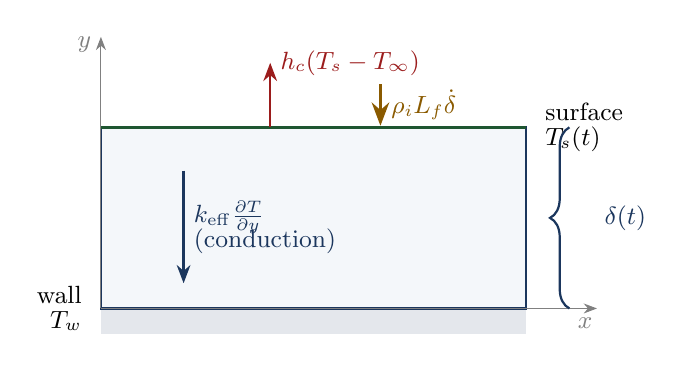
\begin{tikzpicture}[x=1cm,y=1cm,>=Stealth]
  \def\L{5.4}
  \def\Del{2.3}
  % ice layer
  \fill[tint] (0,0) rectangle (\L,\Del);
  \draw[thick,navy] (0,0) rectangle (\L,\Del);
  % wall
  \fill[navy!12] (0,-0.32) rectangle (\L,0);
  \draw[very thick,navy] (0,0)--(\L,0);
  \node[left,align=right,font=\small] at (-0.12,0) {wall\\[-2pt]$\Tw$};
  % surface
  \draw[very thick,greenink] (0,\Del)--(\L,\Del);
  \node[right,align=left,font=\small] at (\L+0.12,\Del) {surface\\[-2pt]$\Ts(t)$};
  % axes
  \draw[->,gray] (0,0)--(0,\Del+1.15) node[left,font=\small] at (0,\Del+1.05) {$y$};
  \draw[->,gray] (0,0)--(\L+0.9,0) node[below,font=\small] at (\L+0.75,0) {$x$};
  % conduction arrow (into ice, toward wall)
  \draw[->,navy,thick] (1.05,1.75)--(1.05,0.32)
     node[midway,right,font=\small,align=left] {$\keff\pd{T}{y}$\\[-2pt](conduction)};
  % convection arrow (to air)
  \draw[->,crimson,thick] (2.15,\Del)--(2.15,\Del+0.82)
     node[right,font=\small] {$h_c(\Ts-\Tinf)$};
  % latent arrow at the surface
  \draw[->,amber,very thick] (3.55,\Del+0.55)--(3.55,\Del+0.02)
     node[midway,right,font=\small] {$\rho_i\Lf\dot\delta$};
  % thickness brace
  \draw[decorate,decoration={brace,amplitude=7pt},thick,navy]
     (\L+0.55,0)--(\L+0.55,\Del)
     node[midway,right=9pt,font=\small] {$\delta(t)$};
\end{tikzpicture}
\caption{One-phase Stefan control volume. Latent heat released at the moving surface is
conducted into the ice toward the cold wall and convected to the ambient. The front
$\delta(t)$ is the unknown moving boundary.}
\label{fig:domain}
\end{figure}

% ============================================================================
\section{Front-fixing (Landau) transformation}\label{sec:transform}
% ============================================================================

Rather than track $\delta(t)$ on a moving mesh, map the ice onto a fixed unit interval,
\begin{equation}
  \xi=\frac{y}{\delta(t)}\in[0,1],
  \qquad \Theta(\xi,t)=T(\delta(t)\xi,t).
\end{equation}
The chain rule gives
\begin{equation}
  \left.\pd{T}{t}\right|_y
  =\pd{\Theta}{t}-\frac{\xi\dot\delta}{\delta}\pd{\Theta}{\xi},
  \qquad
  \pd{T}{y}=\frac1\delta\pd{\Theta}{\xi},
  \qquad
  \pd{^2T}{y^2}=\frac1{\delta^2}\pd{^2\Theta}{\xi^2}.
\end{equation}
Substituting into \eqref{eq:heat} yields the transformed PDE
\begin{equation}\label{eq:transformed}
  \boxed{\;\pd{\Theta}{t}
  =\frac{\alpha}{\delta^2}\pd{^2\Theta}{\xi^2}
   +\frac{\xi\dot\delta}{\delta}\pd{\Theta}{\xi}\;}
\end{equation}
with boundary conditions
\begin{equation}
  \Theta(0,t)=\Tw,\qquad \Theta(1,t)=\Ts,
\end{equation}
and the Stefan condition becomes an ODE for the front,
\begin{equation}\label{eq:frontode}
  \boxed{\;\dot\delta
  =\frac{1}{\rho_i\Lf}\left[
     \frac{\keff}{\delta}\left.\pd{\Theta}{\xi}\right|_{\xi=1}
     +h_c\left(\Ts-\Tinf\right)\right].\;}
\end{equation}

\begin{insightbox}{What the transformation buys}
\begin{itemize}[leftmargin=1.2em,itemsep=2pt]
  \item The Stefan condition is imposed \emph{exactly}: $\delta$ is an ODE state, not a
        level set reconstructed from a smeared latent-heat source.
  \item The moving boundary disappears from the mesh; the grid in $\xi$ is fixed and
        uniform, so standard method-of-lines and V\&V tooling apply.
  \item No artificial mushy-zone width $\varepsilon$ enters the answer.
  \item The cost is a $1/\delta^2$ diffusion coefficient and an extra mesh-motion
        advection term, so the system is stiff and requires an implicit integrator.
\end{itemize}
\end{insightbox}

The advection term $\xi\dot\delta/\delta\,\Theta_\xi$ is the mesh-motion term: a material
point at fixed $y$ drifts toward $\xi=0$ as the layer grows. Its cell P\'eclet number is
\begin{equation}
  \mathrm{Pe}_\xi
  =\frac{|\xi\dot\delta/\delta|\,\Delta\xi}{\alpha/\delta^2}
  =\frac{\xi\dot\delta\,\delta\,\Delta\xi}{\alpha}
  \lesssim 5\times10^{-4}\quad (M=200,\ \text{cases tested here}),
\end{equation}
so central differencing is stable and second-order accurate; no upwinding is required at
the resolutions used here.

% ============================================================================
\section{Numerical discretisation}\label{sec:discretise}
% ============================================================================

\subsection{Grid and state vector}

Use $M=$ \texttt{n\_xi} uniform cells with nodes $\xi_j=j/M$, $j=0,\dots,M$ and
$\Delta\xi=1/M$. Nodes $0$ and $M$ carry the boundary values $\Tw$ and $\Ts$; the
unknowns are the interior temperatures and the front,
\begin{equation}
  \mathbf z=\big(\Theta_1,\dots,\Theta_{M-1},\,\delta\big)^{\!\top}\in\mathbb R^{M}.
\end{equation}

\subsection{Space discretisation}

At interior nodes $j=1,\dots,M-1$,
\begin{align}
  \left(\pd{^2\Theta}{\xi^2}\right)_j
   &\approx \frac{\Theta_{j+1}-2\Theta_j+\Theta_{j-1}}{\Delta\xi^2},\\
  \left(\pd{\Theta}{\xi}\right)_j
   &\approx \frac{\Theta_{j+1}-\Theta_{j-1}}{2\Delta\xi}.
\end{align}
The surface gradient in \eqref{eq:frontode} uses a second-order one-sided stencil,
\begin{equation}
  \left.\pd{\Theta}{\xi}\right|_{\xi=1}
  \approx \frac{3\Theta_M-4\Theta_{M-1}+\Theta_{M-2}}{2\Delta\xi},
\end{equation}
with the same stencil used to evaluate the surface heat balance in the dry branch
(Section~\ref{sec:wetdry}).

The semi-discrete system is
\begin{equation}
  \dot\Theta_j
  =\frac{\alpha}{\delta^2}
     \frac{\Theta_{j+1}-2\Theta_j+\Theta_{j-1}}{\Delta\xi^2}
   +\frac{\xi_j\dot\delta}{\delta}
     \frac{\Theta_{j+1}-\Theta_{j-1}}{2\Delta\xi},
  \qquad j=1,\dots,M-1,
\end{equation}
coupled to \eqref{eq:frontode} for $\dot\delta$.

\subsection{Stiffness and Jacobian structure}

The diffusion coefficient $\alpha/\delta^2$ is the source of stiffness. At the initial
thickness $\delta_0=10\,\mu\mathrm{m}$ and $\alpha\approx1.15\times10^{-6}\,\mathrm{m^2/s}$,
\begin{equation}
  \frac{\alpha}{\delta_0^2}\approx1.2\times10^{4}\ \mathrm{s^{-1}},
\end{equation}
so an explicit scheme would need $\Delta t\lesssim10^{-5}\,\mathrm{s}$ at $M=200$.
The solver therefore defaults to \texttt{BDF} (or \texttt{Radau}/\texttt{LSODA}) and
supplies a Jacobian sparsity pattern: the interior block is tridiagonal, the last column
($\partial/\partial\delta$) is dense because $\delta$ enters every diffusion coefficient,
and the last row couples $\dot\delta$ to the last three temperatures and $\delta$ itself.

\begin{lstlisting}[style=py,caption={Jacobian sparsity pattern supplied to \texttt{solve\_ivp}.},label={lst:jac}]
S = lil_matrix((n, n), dtype=int)
for i in range(m):                 # interior temperature rows
    for j in (i-1, i, i+1):
        if 0 <= j < m:
            S[i, j] = 1
    S[i, m] = 1                    # every T depends on delta
for j in (m-3, m-2, m-1, m):       # front row
    S[m, j] = 1
return S.tocsr()
\end{lstlisting}

\subsection{Initial condition and the $\delta\to0$ singularity}

The transform is singular at $\delta=0$: both $\alpha/\delta^2$ and $1/\delta$ diverge.
The solver starts at a small but finite $\delta_0$ (default $10\,\mu\mathrm{m}$) with a
quasi-steady linear profile. For the pure Stefan case,
\begin{equation}
  \Theta_j(0)=\Tw+(\Tf-\Tw)\,\xi_j .
\end{equation}
For the wet/dry case the surface value is made consistent with the dry Robin balance at
$\delta_0$,
\begin{equation}
  \Ts(0)=\operatorname{clip}\!\left[
    \frac{\mdot_{\mathrm{imp}}\Lf+(\keff/\delta_0)\Tw+h_c\Tinf}
         {\keff/\delta_0+h_c},\;\Tw,\;\Tf\right],
\end{equation}
which removes the startup transient in $\Ts(t)$ visible in an inconsistent initialisation.
The resulting $O(\delta_0^2/\alpha)$ error decays rapidly; at $\delta_0=10\,\mu\mathrm{m}$
and $\alpha\sim10^{-6}\,\mathrm{m^2/s}$ the relaxation time is below $10^{-3}\,\mathrm{s}$.

\subsection{Time integration}

\texttt{solve\_ivp} methods (\texttt{BDF}, \texttt{Radau}, \texttt{LSODA}, \texttt{RK45},
\dots) are supported, as are the fixed-step schemes from \texttt{rosolver.integrators}
(\texttt{beuler}, \texttt{cn}, \texttt{rk4}, \dots). The fixed-step path is what makes the
solver compatible with \texttt{timestep\_study} and the rest of the V\&V stack.
Default tolerances are $\mathrm{rtol}=10^{-8}$, $\mathrm{atol}=10^{-12}$.

% ============================================================================
\section{Wet/dry (Messinger) surface coupling}\label{sec:wetdry}
% ============================================================================

\subsection{Physical idea}

Eq.~\eqref{eq:stefanjump} describes the \emph{maximum} freezing rate the surface heat
balance can sustain with the surface at the freezing point. The actual rate is the
smaller of that capacity and the impingement supply:
\begin{equation}
  \mdot_{\mathrm{ice}}=\min\!\left(\frac{q_{\mathrm{cap}}}{\Lf},\;\mdot_{\mathrm{imp}}\right).
\end{equation}
The two regimes are the classical Messinger rime/glaze split.

\subsection{Capacity and branch selection}

Evaluate the surface-at-freezing capacity using the Dirichlet surface value $\Ts=\Tf$,
\begin{equation}\label{eq:qcap}
  q_{\mathrm{cap}}
  =\frac{\keff}{\delta}
     \frac{3\Tf-4\Theta_{M-1}+\Theta_{M-2}}{2\Delta\xi}
   +h_c\left(\Tf-\Tinf\right),
\end{equation}
and the latent demand of the full supply,
\begin{equation}
  q_{\mathrm{req}}=\mdot_{\mathrm{imp}}\Lf .
\end{equation}

\paragraph{Dry / rime branch ($q_{\mathrm{req}}\le q_{\mathrm{cap}}$).}
All impinging water freezes and the surface cools below freezing. Since the Robin balance
is linear in $\Ts$, the surface temperature is algebraic:
\begin{equation}\label{eq:dryTs}
  \Ts=
  \frac{q_{\mathrm{req}}+h_c\Tinf
        +\dfrac{\keff}{2\delta\Delta\xi}\left(4\Theta_{M-1}-\Theta_{M-2}\right)}
       {\dfrac{3\keff}{2\delta\Delta\xi}+h_c},
\end{equation}
with the front speed set by mass supply,
\begin{equation}
  \dot\delta=\frac{\mdot_{\mathrm{imp}}}{\rho_i},
  \qquad \mdot_{\mathrm{ice}}=\mdot_{\mathrm{imp}},
  \qquad \mdot_{\mathrm{rb}}=0 .
\end{equation}

\paragraph{Wet / glaze branch ($q_{\mathrm{req}}>q_{\mathrm{cap}}$).}
The surface is pinned at the freezing point and cannot freeze the whole supply:
\begin{equation}
  \Ts=\Tf,
  \qquad
  \dot\delta=\frac{q_{\mathrm{cap}}}{\rho_i\Lf},
  \qquad
  \mdot_{\mathrm{rb}}=\mdot_{\mathrm{imp}}-\frac{q_{\mathrm{cap}}}{\Lf}>0 .
\end{equation}

\begin{figure}[htbp]
\centering
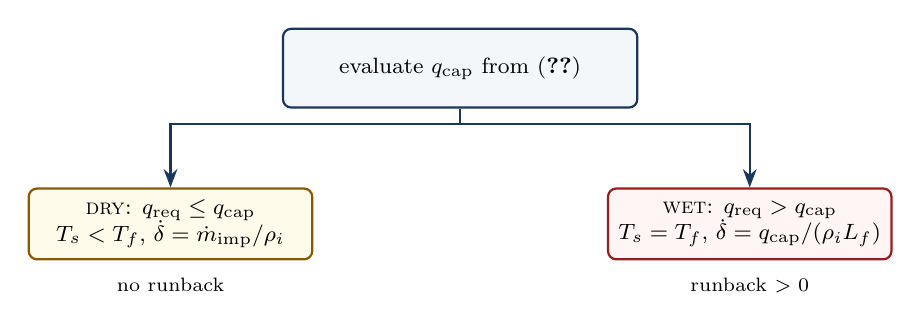
\begin{tikzpicture}[node distance=5mm and 8mm,>=Stealth]
  \node[rectangle,rounded corners=3pt,draw=navy,fill=tint,thick,
        minimum width=4.5cm,minimum height=1.0cm,align=center,font=\footnotesize]
        (cap) {evaluate $q_{\mathrm{cap}}$ from \eqref{eq:qcap}};
  \node[rectangle,rounded corners=3pt,draw=amber,fill=ambertint,thick,
        minimum width=3.6cm,minimum height=0.9cm,align=center,font=\footnotesize,
        below left=10mm and -4mm of cap] (dry) {\branch{dry}: $q_{\mathrm{req}}\le q_{\mathrm{cap}}$\\[-1pt]
        $\Ts<\Tf$, $\dot\delta=\mdot_{\mathrm{imp}}/\rho_i$};
  \node[rectangle,rounded corners=3pt,draw=crimson,fill=red!4,thick,
        minimum width=3.6cm,minimum height=0.9cm,align=center,font=\footnotesize,
        below right=10mm and -4mm of cap] (wet) {\branch{wet}: $q_{\mathrm{req}}>q_{\mathrm{cap}}$\\[-1pt]
        $\Ts=\Tf$, $\dot\delta=q_{\mathrm{cap}}/(\rho_i\Lf)$};
  \draw[->,thick,navy] (cap.south) -- ++(0,-2mm) -| (dry.north);
  \draw[->,thick,navy] (cap.south) -- ++(0,-2mm) -| (wet.north);
  \node[below=1mm of dry,font=\scriptsize,align=center] {no runback};
  \node[below=1mm of wet,font=\scriptsize,align=center] {runback $>0$};
\end{tikzpicture}
\caption{Surface branch selection. The vector field is continuous at the switch: setting
$q_{\mathrm{req}}=q_{\mathrm{cap}}$ makes the dry and wet front speeds equal.}
\label{fig:branch}
\end{figure}

\subsection{Continuity at the switch}

At the crossover $q_{\mathrm{req}}=q_{\mathrm{cap}}$, the dry branch gives
\begin{equation}
  \dot\delta=\frac{\mdot_{\mathrm{imp}}}{\rho_i}
  =\frac{q_{\mathrm{req}}}{\rho_i\Lf}
  =\frac{q_{\mathrm{cap}}}{\rho_i\Lf},
\end{equation}
which is exactly the wet-branch value. Hence $\dot\delta$ and $\Ts$ are continuous, and
only the derivative jumps. The ODE is $C^0$ but not $C^1$, which \texttt{BDF} handles by
reducing order locally; the tests confirm that the front remains accurate through the
switch.

\begin{insightbox}{What the coupling does and does not add}
The switch adds the \emph{regime} distinction and a runback diagnostic. Runback is a
per-unit-area mass flux; the lumped film that stores and drains the excess water is
introduced in Section~\ref{sec:film}.
\end{insightbox}

% ============================================================================
\section{Hybrid accretion/shedding coupling}\label{sec:hybrid}
% ============================================================================

The event-driven machinery in \texttt{rosolver.numerical} uses terminal
\texttt{solve\_ivp} events on a scalar state. The front position $\delta$ is already an
explicit ODE state in the transformed system, so it can be reused without changing the
PDE discretisation. A shedding threshold is packaged as
\begin{equation}
  g(t,\delta)=\delta-\delta_{\mathrm{crit}},
  \qquad
  \texttt{stefan\_shedding\_event}(\delta_{\mathrm{crit}},s),
\end{equation}
with upward crossing $g'=\dot\delta>0$. At the event time $t_e$ integration stops, the
state is taken from \texttt{sol.y\_events}, and the ice thickness is reset to
\begin{equation}\label{eq:shedreset}
  \delta(t_e^+)=(1-s)\,\delta(t_e^-),\qquad 0\le s\le 1,
\end{equation}
the retained ice is the inner $(1-s)$ fraction of the old layer. The temperature field is
resampled from $\xi_{\mathrm{old}}=\xi(1-s)$ onto the new grid, so physical temperatures
are continuous at the reset; any surface film leaves with the shed slab. Integration
restarts at $t_e+10^{-9}\,\mathrm{s}$ and repeats until $t_{\mathrm{end}}$ or
\texttt{max\_events}. The returned \texttt{HybridStefanSolution} carries one
\texttt{SheddingRecord} per event with the pre/post front positions and the shed amount.

\begin{insightbox}{Why an explicit reset, not a source term}
A shed event is a discontinuity in ice mass, so it cannot be represented by a smooth
source in the Stefan condition. A terminal event keeps the front condition exact between
events and makes the mass loss exactly $s\,\delta(t_e^-)$.
\end{insightbox}

% ============================================================================
\section{Runback film and the complete surface-energy closure}\label{sec:film}
% ============================================================================

Let $h_f(t)$ be a lumped liquid-film thickness on the ice surface. Film mass conservation
reads
\begin{equation}\label{eq:filmmass}
  \rho_w\dot h_f=\mdot_{\mathrm{imp}}+\mdot_{\mathrm{in}}-\mdot_{\mathrm{ice}}
                 -\mdot_{\mathrm{evap}}-\frac{\rho_w h_f}{\tau_d},
\end{equation}
where $\tau_d$ is the drainage time. The surface energy balance gains the impingement
sensible enthalpy, impact kinetic heating and evaporation,
\begin{align}\label{eq:surfacefull}
  \frac{\keff}{\delta}\left.\pd{\Theta}{\xi}\right|_1
   +h_c(\Ts-\Tinf)
   +\underbrace{\mdot_{\mathrm{imp}}c_w(\Ts-\Timp)}_{\text{sensible}}
   +\underbrace{\mdot_{\mathrm{evap}}L_v-\tfrac12\mdot_{\mathrm{imp}}V_{\mathrm{imp}}^2}_{\text{evaporation / kinetic}}
   &=\mdot_{\mathrm{ice}}\Lf .
\end{align}
Evaluating \eqref{eq:surfacefull} at $\Ts=\Tf$ generalises the capacity \eqref{eq:qcap} to
\begin{equation}\label{eq:qcapfull}
  q_{\mathrm{cap}}=\frac{\keff}{\delta}
   \frac{3\Tf-4\Theta_{M-1}+\Theta_{M-2}}{2\Delta\xi}
   +h_c(\Tf-\Tinf)+\mdot_{\mathrm{imp}}c_w(\Tf-\Timp)
   +\mdot_{\mathrm{evap}}L_v-\tfrac12\mdot_{\mathrm{imp}}V_{\mathrm{imp}}^2 .
\end{equation}

\paragraph{Branch selection without a thickness switch.}
The branch is chosen by the energy criterion alone:
\begin{equation}\label{eq:wetswitch}
  \texttt{wet}\iff \mdot_{\mathrm{imp}}\Lf>q_{\mathrm{cap}} .
\end{equation}
A positive film supplies extra water
$\mdot_{\mathrm{avail}}=\mdot_{\mathrm{imp}}+\rho_w h_f/\tau_f$ with freeze-out time
$\tau_f$, but it does \emph{not} by itself pin $\Ts=\Tf$. Hence
\begin{equation}\label{eq:filmclosure}
  \mdot_{\mathrm{ice}}=\min\!\left(\frac{q_{\mathrm{cap}}}{\Lf},\mdot_{\mathrm{avail}}\right),
  \qquad
  \Ts=\begin{cases}
    \Tf, & \texttt{wet},\\[3pt]
    \Ts^{\mathrm{dry}}, & \texttt{dry},
  \end{cases}
\end{equation}
where the dry surface temperature is the algebraic Robin solution
\begin{equation}\label{eq:dryTsfull}
  \Ts^{\mathrm{dry}}=
  \frac{\mdot_{\mathrm{ice}}\Lf+h_c\Tinf+\mdot_{\mathrm{imp}}c_w\Timp
       +\frac{\keff}{2\delta\Delta\xi}(4\Theta_{M-1}-\Theta_{M-2})}
       {\frac{3\keff}{2\delta\Delta\xi}+h_c+\mdot_{\mathrm{imp}}c_w}.
\end{equation}
At the crossover $q_{\mathrm{req}}=q_{\mathrm{cap}}$, both branches give
$\mdot_{\mathrm{ice}}=\mdot_{\mathrm{imp}}$ and $\Ts=\Tf$. The vector field is therefore
$C^0$ across the switch. Continuity matters numerically: an earlier criterion
$\texttt{wet}\iff h_f>0$ made $\Ts$ jump at $h_f=0$, and \texttt{BDF} stalled at film
exhaustion. With \eqref{eq:wetswitch} the film drains smoothly to zero, and a
pre-existing film on a thin ice layer simply freezes back on the $O(\tau_f)$ timescale.

In the wet steady state $\dot h_f=0$ and \eqref{eq:filmmass} yields
\begin{equation}\label{eq:filmsteady}
  h_f^*=\frac{\tau_d}{\rho_w}\left(\mdot_{\mathrm{imp}}
        -\frac{q_{\mathrm{cap}}}{\Lf}-\mdot_{\mathrm{evap}}\right)>0 ,
\end{equation}
which is positive precisely in the energy-limited regime. The freezing fraction
$n=\mdot_{\mathrm{ice}}/(\mdot_{\mathrm{imp}}+\mdot_{\mathrm{in}})$ and the drainage flux
$\rho_w h_f/\tau_d$ are reported on the solution.

\begin{insightbox}{Enthalpy sign convention}
Supercooled droplets ($\Timp<\Tf$) and evaporation \emph{increase} the required heat
removal and therefore reduce the freezing rate; impact kinetic energy does the opposite.
The numerical tests check each term against its own flux magnitude
$\mdot_{\mathrm{imp}}c_w(\Tf-\Timp)$, $\mdot_{\mathrm{evap}}L_v$ and
$\tfrac12\mdot_{\mathrm{imp}}V_{\mathrm{imp}}^2$.
\end{insightbox}

% ============================================================================
\section{Verification and results}\label{sec:verify}
% ============================================================================

\subsection{Exact Neumann similarity solution ($h_c=0$)}

For $h_c=0$, constant properties and a fixed wall temperature, the one-phase problem
admits the similarity solution
\begin{equation}\label{eq:neumannT}
  T(y,t)=\Tw+(\Tf-\Tw)\frac{\operatorname{erf}\eta}{\operatorname{erf}\lambda},
  \qquad
  \eta=\frac{y}{2\sqrt{\alpha t}},
\end{equation}
\begin{equation}\label{eq:neumannfront}
  \delta(t)=2\lambda\sqrt{\alpha t},
\end{equation}
where $\lambda$ solves
\begin{equation}\label{eq:lambda}
  \boxed{\;\lambda e^{\lambda^2}\operatorname{erf}\lambda
  =\frac{\mathrm{Ste}}{\sqrt\pi},\qquad
  \mathrm{Ste}=\frac{c_p(\Tf-\Tw)}{\Lf}.\;}
\end{equation}
Equation~\eqref{eq:lambda} is solved with Brent's method on a monotone residual; the
small-$\mathrm{Ste}$ limit is $\lambda\simeq\sqrt{\mathrm{Ste}/2}$, which reproduces the
familiar $\delta\sim\sqrt{2\alpha\,\mathrm{Ste}\,t}$ law.

\begin{resultbox}{Exact front validation}
With $k=2.22\,\mathrm{W\,m^{-1}K^{-1}}$, $\rho=917\,\mathrm{kg\,m^{-3}}$,
$c_p=2100\,\mathrm{J\,kg^{-1}K^{-1}}$, $\Lf=3.34\times10^{5}\,\mathrm{J\,kg^{-1}}$,
$\Tw=-6\,^\circ\mathrm{C}$, $\Tf=0\,^\circ\mathrm{C}$, $h_c=0$:
\[
  \mathrm{Ste}=0.037725,\qquad \lambda=0.13648875,
\]
\[
  \delta_{\mathrm{PDE}}(1\,\mathrm{h})=17.585722\,\mathrm{mm},\qquad
  \delta_{\mathrm{Neumann}}(1\,\mathrm{h})=17.585724\,\mathrm{mm},
\]
\[
  \text{relative front error}=1.6\times10^{-7}.
\]
\end{resultbox}

\subsection{Quasi-steady reduction ($\mathrm{Ste}\to0$)}

In the limit $\mathrm{Ste}\to0$ the profile is linear and the Stefan condition reduces to
\begin{equation}\label{eq:qs}
  \rho_i\Lf\,\delta\dot\delta
  =\keff(\Tf-\Tw)+h_c(\Tf-\Tinf)\,\delta .
\end{equation}
Writing $q=\delta^2$ gives the scalar ODE
\begin{equation}
  \dot q=2\kappa+2\beta\sqrt q,
  \qquad
  \kappa=\frac{\keff(\Tf-\Tw)}{\rho_i\Lf},
  \qquad
  \beta=\frac{h_c(\Tf-\Tinf)}{\rho_i\Lf},
\end{equation}
which is integrated with \texttt{BDF} and used as a reference curve. The two terms in
\eqref{eq:qs} identify a crossover thickness
\begin{equation}
  \delta^\ast=\frac{\keff(\Tf-\Tw)}{h_c(\Tf-\Tinf)} ,
\end{equation}
below which conduction controls ($\delta\sim\sqrt t$) and above which convection controls
($\delta\sim t$).

Table~\ref{tab:quasi} compares the full PDE with \eqref{eq:qs} for the convective case
$\Tw=\Tinf=-4.13\,^\circ\mathrm{C}$, $\Tf=-1.18\,^\circ\mathrm{C}$, $h_c=160\,
\mathrm{W\,m^{-2}K^{-1}}$, for which $\delta^\ast=13.875\,\mathrm{mm}$.

\begin{table}[htbp]
\centering
\caption{Full front-fixed PDE versus the quasi-steady reduction over 24 hours. The
$O(\mathrm{Ste})$ gap, with $\mathrm{Ste}=0.0185$, is the expected transient correction.}
\label{tab:quasi}
\begin{tabular}{rrrr}
\toprule
$t$ [h] & $\delta_{\mathrm{PDE}}$ [mm] & $\delta_{\mathrm{quasi}}$ [mm] & difference [\%]\\
\midrule
 1  &  16.289 &  16.351 & 0.38 \\
 6  &  55.395 &  55.648 & 0.46 \\
12  &  94.721 &  95.182 & 0.48 \\
24  & 168.061 & 168.923 & 0.51 \\
\bottomrule
\end{tabular}
\end{table}

\begin{figure}[htbp]
\centering
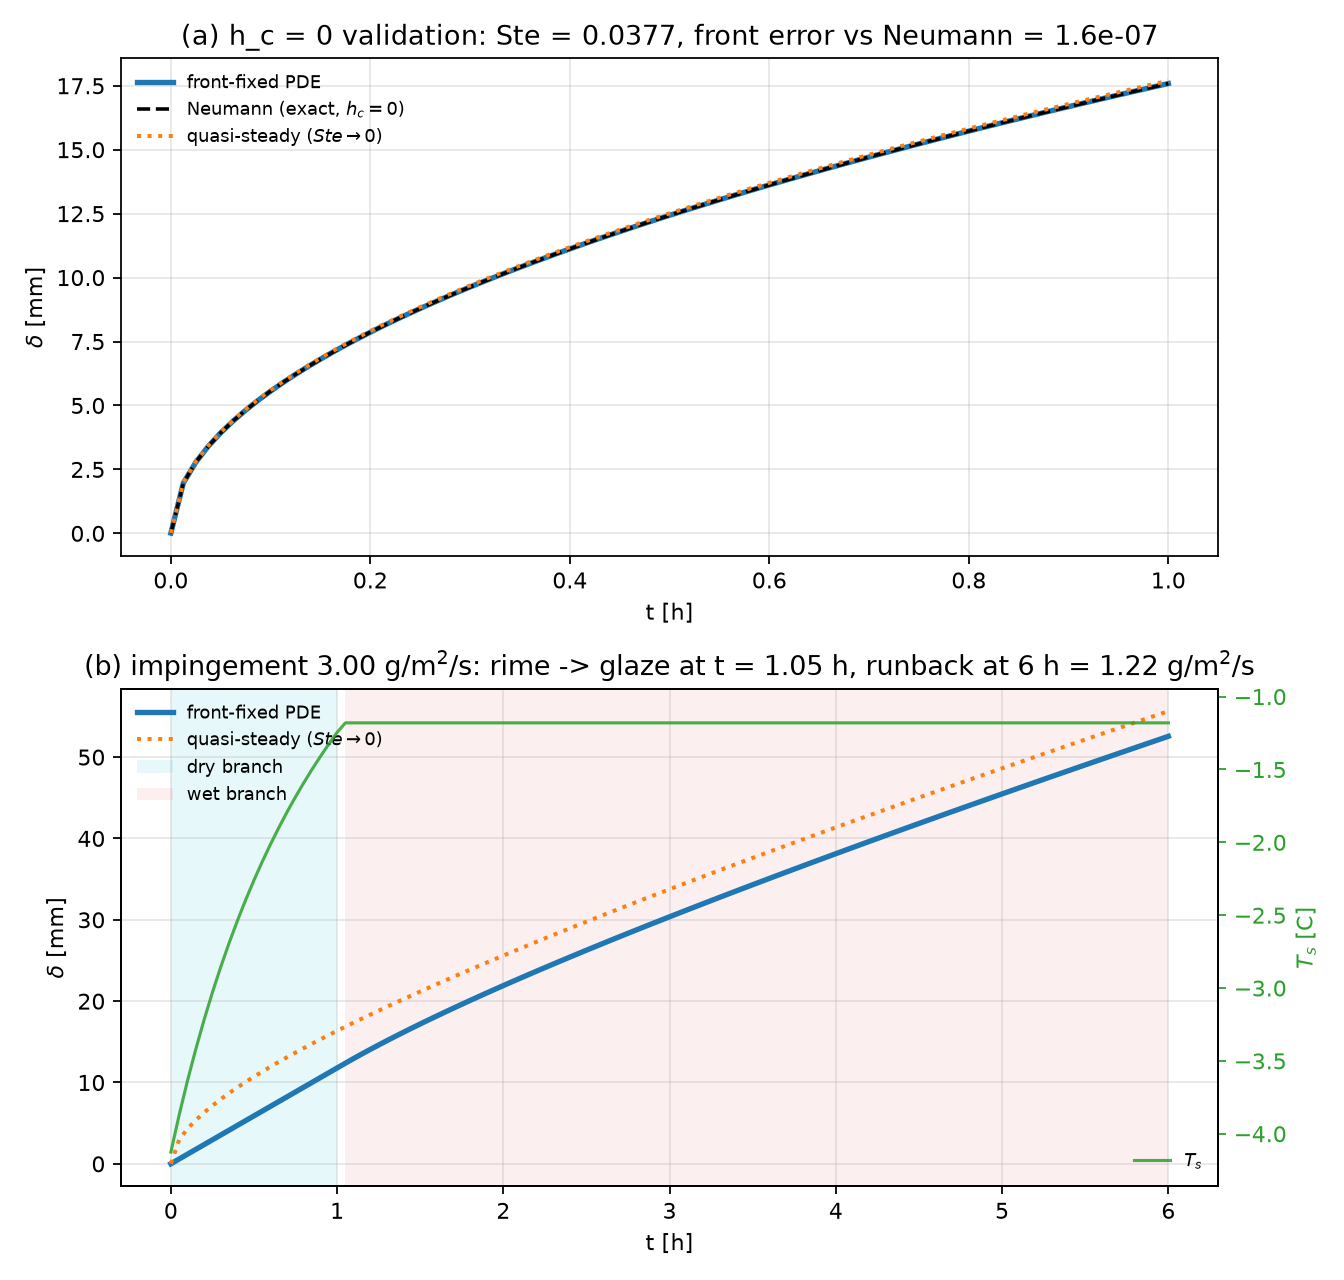
\includegraphics[width=0.96\textwidth]{stefan_front_validation.png}
\caption{Generated by \texttt{python -m examples.stefan\_validation}.
(a) $h_c=0$: front-fixed PDE against the exact Neumann solution and the quasi-steady
reduction; the front error is $1.6\times10^{-7}$.
(b) Finite impingement $\mdot_{\mathrm{imp}}=3\,\mathrm{g\,m^{-2}s^{-1}}$: the
rime$\to$glaze transition at $t=1.05\,\mathrm{h}$, with the wet-limit quasi-steady
reference and the surface temperature $\Ts(t)$ on the right axis. The dry branch is shaded
cyan and the wet branch red.}
\label{fig:validation}
\end{figure}

\subsection{Spatial convergence and branch tests}

The spatial stencils are second-order; the test verifies that refining
$M\in\{50,100,200\}$ reduces the front error monotonically toward the Neumann value.
This is a monotonicity check, not a measured convergence rate: with the default time
tolerances the error at $M=200$ is already at the tolerance floor, and tightening
$\mathrm{rtol}$ to $10^{-12}$ leaves a residual $\sim4\times10^{-9}\,\mathrm{m}$ for
$M\ge400$ set by the finite $\delta_0$ start rather than by the mesh. The wet/dry tests
additionally verify:
\begin{itemize}[leftmargin=1.4em,itemsep=2pt]
  \item the dry branch is exactly mass-limited, $\delta(t)=\delta_0+\mdot_{\mathrm{imp}}t/\rho_i$;
  \item the wet branch with abundant supply reproduces the pure Stefan model to solver tolerance;
  \item the switch occurs at $\Ts=\Tf$ and the freezing flux is continuous there;
  \item runback is zero in the dry branch and increases monotonically after the switch.
\end{itemize}

\begin{table}[htbp]
\centering
\caption{Rime$\to$glaze demonstration at $\mdot_{\mathrm{imp}}=3\,\mathrm{g\,m^{-2}s^{-1}}$.}
\label{tab:wetdry}
\begin{tabular}{rrrlrr}
\toprule
$t$ [h] & $\delta$ [mm] & $\Ts$ [$^\circ$C] & branch &
freezing [g\,m$^{-2}$s$^{-1}$] & runback [g\,m$^{-2}$s$^{-1}$]\\
\midrule
0.5 &  5.899 & $-2.260$ & dry & 3.000 & 0.000 \\
1.0 & 11.788 & $-1.246$ & dry & 3.000 & 0.000 \\
2.0 & 21.915 & $-1.180$ & wet & 2.294 & 0.706 \\
4.0 & 38.127 & $-1.180$ & wet & 1.916 & 1.084 \\
6.0 & 52.553 & $-1.180$ & wet & 1.775 & 1.225 \\
\bottomrule
\end{tabular}
\end{table}

% ============================================================================
\section{Software implementation}\label{sec:software}
% ============================================================================

\subsection{Module map}

\begin{table}[htbp]
\centering
\caption{Files added or extended by this implementation.}
\label{tab:files}
\begin{tabularx}{\textwidth}{@{}lX@{}}
\toprule
File & Contents \\
\midrule
\texttt{rosolver/phasechange.py} &
\texttt{Stefan1D} (model, RHS, branch closure, Jacobian sparsity, driver),
\texttt{StefanSolution} (queries and diagnostics), \texttt{neumann\_lambda},
\texttt{neumann\_delta}, \texttt{quasi\_steady\_delta}. \\
\texttt{rosolver/simulate.py} &
\texttt{plot\_stefan}: front against Neumann and quasi-steady references, optional
wet/dry shading and $\Ts$ twin axis; draws into a new figure or a supplied axis. \\
\texttt{rosolver/\_\_init\_\_.py} & Public exports. \\
\texttt{examples/stefan\_validation.py} & Generates
\texttt{figures/stefan\_front\_validation.png}. \\
\texttt{tests/test\_phasechange.py} & 16 tests covering exactness, convergence,
branch logic, guards and plotting. \\
\bottomrule
\end{tabularx}
\end{table}

\subsection{Public API}

\begin{lstlisting}[style=py,caption={Typical use.},label={lst:api}]
from rosolver import Stefan1D, plot_stefan

# 1. Exact Neumann validation (h_c = 0)
st = Stefan1D(T_wall=-6.0, T_f=0.0, h_c=0.0, n_xi=200)
sol = st.solve(3600.0, delta0=1e-5)
print(sol.delta[-1], float(st.neumann_delta(3600.0)))   # ~1e-7 relative

# 2. Convective surface with SnowTek/WINICE numbers
st = Stefan1D(T_wall=-4.13, T_inf=-4.13, T_f=-1.18, h_c=160.0)
sol = st.solve(86400.0, delta0=1e-5)
y, T = sol.profile()
print(sol.summary(), st.quasi_steady_delta(86400.0, 1e-5))

# 3. Rime -> glaze with finite impingement
st = Stefan1D(T_wall=-4.13, T_inf=-4.13, T_f=-1.18,
              h_c=160.0, mdot_imp=3e-3)
sol = st.solve(6 * 3600.0, delta0=1e-5)
print(sol.branch[-1], sol.runback(-1))
plot_stefan(sol, st, path="stefan_wetdry.png", show_surface=True)
\end{lstlisting}

\texttt{StefanSolution} stores the front, the full temperature profile at each snapshot,
the surface temperature, the freezing mass flux and the branch label. Convenience queries
include \texttt{profile()}, \texttt{delta\_at()}, \texttt{temperature\_at()},
\texttt{front\_gradient()} and \texttt{runback()}.

\subsection{Test summary}

\begin{resultbox}{Verification status}
\begin{itemize}[leftmargin=1.2em,itemsep=2pt]
  \item \texttt{test\_phasechange.py}: 16/16 passed.
  \item Full repository suite: 55/55 passed.
  \item Exact Neumann agreement: $1.6\times10^{-7}$ relative.
  \item PDE vs quasi-steady over 24\,h: $0.38$--$0.51\%$ at $\mathrm{Ste}=0.0185$,
        consistent with the $O(\mathrm{Ste})$ truncation of the reduction.
\end{itemize}
\end{resultbox}

% ============================================================================
\section{Limitations and extensions}\label{sec:limits}
% ============================================================================

\begin{enumerate}[leftmargin=1.5em,itemsep=3pt]
  \item \textbf{Single phase, 1D.} The model is one-phase and one-dimensional. Remelting,
        multiple fronts, or 3D geometries require the enthalpy (apparent heat capacity)
        formulation on a fixed grid, which trades the exact front for an
        $\varepsilon$-smeared one.
  \item \textbf{Conductivity closure.} $\keff(\phi)$ is taken constant. The sheet gives
        no evolution equation for the porosity $\phi$, so eq.~(3.4) is underdetermined if
        $\keff$ is allowed to vary. A future extension is
        $\keff=\keff(\phi)$ coupled to a WINICE constitutional-supercooling porosity
        equation, or Bayesian calibration of a constant $\keff$ following the UQ plan of
        the equation sheet (Section~6).
  \item \textbf{Dry surface closure.} The dry branch uses the quasi-steady Robin balance
        and has no surface heat capacity. This is accurate to $O(\mathrm{Ste})$ here
        ($\approx2\%$), but a finite surface capacitance would be needed for very fast
        transients.
  \item \textbf{Lumped film.} Section~\ref{sec:film} stores runback water in a single
        thickness $h_f(t)$; there is no spatial film transport or rivulet formation.
        The freeze-out time $\tau_f$ is a regularisation, not a calibrated property.
  \item \textbf{Startup singularity.} The front-fixing map is singular at $\delta=0$; the
        solver starts at $\delta_0>0$. The choice of $\delta_0$ only affects a transient
        shorter than $10^{-3}\,\mathrm{s}$ at the parameters used.
\end{enumerate}

\subsection*{Extensions implemented}

The two extensions recommended in the first version of these notes are now in place:
\begin{enumerate}[leftmargin=1.5em,itemsep=2pt]
  \item \textbf{Hybrid shedding.} \texttt{Stefan1D.solve\_with\_shedding} uses a
        \texttt{SheddingEventSpec} with margin $\delta-\delta_{\mathrm{crit}}$
        (Section~\ref{sec:hybrid}).
  \item \textbf{Runback film.} The lumped film ODE \eqref{eq:filmmass} and the full
        surface-energy closure \eqref{eq:surfacefull}, including impingement enthalpy,
        are integrated as additional states (Section~\ref{sec:film}).
\end{enumerate}

\subsection*{Remaining next steps}

Two further extensions are natural but not yet implemented:
\begin{enumerate}[leftmargin=1.5em,itemsep=2pt]
  \item Distribute the film over the surface (a 1D shallow-water/rivulet model) instead of
        one lumped thickness, so that spatially varying shedding can be represented.
  \item Close $\keff(\phi)$ with the WINICE porosity equation and calibrate it with the
        Bayesian U\&Q workflow on the equation sheet.
\end{enumerate}

% ============================================================================
\begin{thebibliography}{9}
% ============================================================================

\bibitem{landau}
H.~G. Landau,
\emph{Heat conduction in a melting solid},
Quarterly of Applied Mathematics \textbf{8} (1950) 81--94.

\bibitem{carslaw}
H.~S. Carslaw and J.~C. Jaeger,
\emph{Conduction of Heat in Solids}, 2nd ed.,
Oxford University Press, 1959, ch.~XI.

\bibitem{messinger}
B.~L. Messinger,
\emph{Equilibrium temperature of an unheated icing surface as a function of air speed},
Journal of the Aeronautical Sciences \textbf{20} (1953) 29--42.

\bibitem{oti}
OTI interview technical equation cheat-sheet,
\texttt{docs/refs/oti\_equation\_cheat\_sheet.md}, eqs.~3.1--3.4.

\bibitem{asme}
ASME V\&V 20--2009,
\emph{Standard for Verification and Validation in Computational Fluid Dynamics and Heat
Transfer}, American Society of Mechanical Engineers, 2009.

\end{thebibliography}

\end{document}
